\documentclass[10pt,letterpaper,twocolumn]{article}
\usepackage{amsmath}
\usepackage{graphicx} 
\title{Flash Matting In Natural Images}
\author{
        Per Karlsson \\
                perk@stanford.edu
}
\date{\today}

\begin{document}
\maketitle{}

\begin{abstract}
I have tried to implement flash matting in natural images, where the idea is that anybody should be able to perform matting, i.e remove foreground from background, no matter where they are and how the background looks like. To solve this, we will need a trimap defining guaranteed areas of foreground, background and a region where we want to perform an alpha approximation. A modified version Bayesian matting will be used to approximate the alpha over this area.
\end{abstract}

\section{Introduction}
The main goal with the matting problem is to extract a foreground from a picture's background as accurate as possible. We define the foregrounds opacity at each pixel with the help of an alpha channel, which will be zero everywhere where the foreground does not exist. Areas that are completely covered by a foreground has the maximum alpha value (that depends on the implementation) and in transitions between foreground and background there exists a range of different alpha values from min to max. This range is important to make it the matting look natural, where a hard cut off can create unrealistic behavior (for example in hair, fur).
\\
Matting is commonly used to capture and image or sequence of images in one environment and later in a post-production stage change the background to make it look like the original captured in that environment. This can be done by hand entirely but required a lot of work and can be different from case to case. This paper is based on a project work in cs478 Computational Photography where I tried to implement an automatic generation of alpha matting without to much extra work by the user. My idea was originally to try to implement this on a handheld tablet device with a built-in camera. The more I worked with the project, the more I realized that alpha matting is extremely sensitive to input data and small changes in input data can lead to huge differences in the output.
\\
The are different categories of matting problems. I have chosen to focus on the natural images background, i.e in original scenes where the background can have an arbitrary color spectrum. This means that the user can take a photo pretty much everywhere and will still be able apply the algorithm to remove the object from the background.

\section{Background}
One of the classic and early matting solutions was to create a big screen in a solid base color and put it behind the object[1] (from the camera's point of view). If this base color is not common in the object's spectrum of colors, then this base color can be removed from the input in a fairly easy manner. This technique requires the users to have a photo studio with proper lighting to remove smearing at the borders. For a sequence of images, this is still the most common method to use. For single images, this has been a popular research area for the last ten years. In 2001[2] presented a way to use probability to model color distribution and alpha generation. This method required a trimap that divided the image into three regions, i.e the user had to specify regions where they were completely guaranteed that pixels either belong to the foreground or the background and a final region of unknown and to be decided pixels. By trying to maximize the likelihood of colors and alpha, all pixels in the unknown area were eventually updated. The method presented in this paper produced poor results in environments where the color vectors in the foreground and background objects were similar. Trying to find a modified and more stable approach, [3] released a paper where they shoot two photos directly after each other, one with flash and one without. If the flash only hits the object in the foreground and light it up, the background will look approximately the same in both pictures while the object in focus looks differently. I tried to implement the methods discussed in this paper as my final project.

\section{Method}
\subsection{Trimap}
According to [3], the flash matting approach can automatically generate a trimap for you. The algorithm is simple but I ended up using a user-defined trimap in the end (see Discussion). The algorithm for the automatic trimap is the following:
\begin{enumerate}
\item Generate histogram of intensities
\item Smooth the histogram with a gaussian kernel ($\sigma^2 = 7$).
\item Set $T_1$ to the first local minimum, starting from top intensity
\item Mark all pixels above $T_1$ as $R_1$.
\item Set $T_1$ to $0.6T$.
\item Mark all pixels above $0.6T$ as $R_2$.
\item Remove regions from $R_2$ that do not overlap anything in $R_1$.
\item Merge remaining $R_1$ and $R_2$ as $R$. This is your area for the known foreground.
\item Dilate $R$ with a constant width, to create the thick border $R_{unknown}$. This is the area of unknown pixels
\item The rest of the image can be marked as known background.
\end{enumerate}


\subsection{Flash matting equations}
A static foreground image taken without a flash can be divided into a foreground and a background part according to this equation:
\begin{equation}
I = \alpha F + (1 - \alpha) B
\label{eq:first}
\end{equation}
where $\alpha$ is the alpha channel. With just one image as input, we don't know the values of $F$, $B$ and $\alpha$ everywhere. In the same manner, we can define a similar equation for the flash image
\begin{equation}
I^f = \alpha F^f + (1 - \alpha) B^f
\end{equation}
where $\alpha$ is the same $\alpha$ as in equation \ref{eq:first}. The light radiance from a point light $\L$ is defined as:
\begin{equation}
E = c_i * r^{-2} * cos \theta
\label{eq:intensity}
\end{equation}
where $c_i$ is a light and material constant, $r$ is the distance to the point light and $\theta$ is the angle between incoming and surface normal. If the flash of a camera is treated as point light source, then equation \ref{eq:intensity} tells us that objects far away from the camera will quadratically gain less intensity. Basically, this means that unless our background is close to the camera, it won't be affected much by the camera flash and we can make the assumptions:
\begin{equation}
B^f \approx B\\
\end{equation}
\begin{equation}
I^f \approx \alpha F^f + (1-\alpha) B
\end{equation}
We can now derive the foreground flash matting equation:
\begin{equation}
I^d = I^f - I \approx \alpha F^d
\end{equation}

For objects with hard and solid edges, implementing a simple matting can be done in a straight forwarded way. By just taking the difference between the flash and no flash image, background colors will cancel each other and you are left with an area of only foreground pixels. Since the object had hard edges, you don't have to care about alpha at the boundaries. Applying a $2-3$ pixels wide smoothing kernel can be added if the foreground edge looks to rough in the new composition. The hardest part is obviously to create matting for complex foregrounds with complex natural background and that is what I tried to implement. To only let the foreground be defined by differences in $I$ and $I^f$ is going have jagged artefacts in the boundaries.

\subsection{Modified Bayesian matting}
To estimate the alpha in the unknown areas of the trimap, we are going to use a modified version of the Bayesian matting introduced in [2]. To start with, the only thing we know about an unknown pixel, is its value in the no flash image $I$ and in the difference image $I^d$. Given this, we want to maximize the probability of all the colors and the alpha in this pixel:
\begin{equation}
\arg\max_{\alpha, F, F^d, B} P(a,F,F^d,B|I,I^d)
\end{equation}
\begin{equation}
\arg\max_{\alpha, F, F^d, B} P(I|\alpha, F, B)P(I^d|\alpha F^d)P(F)\\P(B)P(F^d)
\label{maxi}
\end{equation}
In equation \ref{maxi}, the $P(I,I^d)$ is constant and removed since we are only interested in what values that maximizes the function. $P(\alpha)$ is also removed since we approximate any alpha to be as likely as any other alpha. To maximize this, we use maximum log likelihood to get rid of the multiplications and we are left with:

\begin{align*}
\arg\max_{\alpha, F, F^d, B}  L(I|\alpha,F,B) + L (I^d|\alpha, F^d) + L(F) +  \\L(B) + L(F^d)
\end{align*}
where $L(x)$ is the log of probability of $P(x)$. To find the maximum, we need to make 10 partial derivatives (that is how many unknowns we have, 3 for each $F$, $B$ and $F^d$) and set them equal to zero. [2] solved this by treating $\alpha$ and the colors $F,B,F^d$ constant in turns. By doing this, the partial derivatives equal to zero can be solved by the following iterative formulas:
\begin{equation}
\alpha = \frac{(F-B)^T(I-B) + F^{d^T}I^d}{(F-B)^T(F-B) + F^{d^T}F^d}
\label{eq:alpha}
\end{equation}
$$ K = 
\begin{bmatrix}
1 & 0 & 0 \\
0 & 1 & 0 \\
0 & 0 & 1 \\
\end{bmatrix} \cdot\alpha^2/\sigma^2
$$

$$
L = 
\begin{bmatrix}
1 & 0 & 0 \\
0 & 1 & 0 \\
0 & 0 & 1 \\
\end{bmatrix} \cdot\alpha(1-\alpha)/\sigma^2
$$
$$
\begin{bmatrix}
\Sigma_F^{-1} + K & L & 0 \\
L & \Sigma_B^{-1} +  K & 0 \\ 
0 & 0 & \Sigma_{F^d}^{-1} +  K
\end{bmatrix}
\begin{bmatrix}
F\\
B\\
F^d
\end{bmatrix}
=
$$
$$
\begin{bmatrix}
\Sigma_F^{-1}\bar{F} + I\alpha/\sigma^2 \\
\Sigma_B^{-1}\bar{F} + I(1-\alpha)/\sigma^2 \\
\Sigma_{F^d}^{-1}\bar{F^d} + I\alpha/\sigma^2 \\
\end{bmatrix}
$$

where

\begin{equation}
\bar{F} = \frac{1}{W}\sum_{i\in{N}} \omega_i F_i
\label{eq:mean}
\end{equation}
\begin{equation}
\Sigma_F = \frac{1}{W}\sum_{i\in{N}} \omega_i (F_i - \bar{F})(F_i - \bar{F})^T
\label{eq:cov}
\end{equation}

$\Sigma_B$,  $\Sigma_{F^d}$, $\bar{B}$, $\bar{F^d}$ can be derived in the same way as $F$ in equations \ref{eq:mean} and \ref{eq:cov}. $\omega$ is the weight that depends on the opacity of nearby pixels and distance to them:
\begin{equation}
\omega_i = \alpha_i^2e^{-\frac{\Delta_i}{2\sigma^2}}
\end{equation}
When you are calculating mean and covariance matrices for background, you should use the following formula instead for weights:
\begin{equation}
\omega_i = (1-\alpha_i)^2e^{-\frac{\Delta_i}{2\sigma^2}}
\end{equation}
 Since I set the noise in $I$ to the same noise as in $I^d$, the $\sigma$'s cancel in equation \ref{eq:alpha}. Equations \ref{eq:alpha} and \ref{eq:axb} can not be solved at the same time. You start by initating $F$, $B$ and $F^d$ in every pixel by the weigthed mean values (equation \ref{eq:mean}). Then you update first equation \ref{eq:alpha} and later equation \ref{eq:axb}. You keep doing this until $\alpha$ has converged to some small value $\epsilon$ or for a fixed amount of iterations.

\section{Implementation}
The first thing I do is to read the Flash $I^f$ and no flash $I$ image pair from image files. With those two, I can create the difference image $I^d$. Next step is to load the custom made trimap. Once the trimap is loaded, I can specify foreground and background pixel values ($F$, $B$ and $F^d$) in known regions. I add all unknown pixel coordinates in a \texttt{std::set}.
\\
Next step is to find the contour of the unknown region. For this, I create a \texttt{std::queue} of pixel coordinates. Every pixel that has at least one neighbor that is not in the unknown region gets added to this queue. Once the queue is filled with the contour, I process the pixels one by one and update them according to equation \ref{eq:alpha}. I run the updates a fixed number of iterations for each pixel since it is easier to control the time complexity of the algorithm (see Discussion). If $\alpha$ gets outside the range of $0$ to $1$ or a pixel $0$ to $255$, I simply clamp the values to this range.
\\
A very time consuming part is to calculate the mean colors and inverse covariance matrix at each unknown pixel. First, you have to find the neighboring pixels that have the same type as the mean color or covariance matrix you are calculating for or previous updated unknown pixels. For example, if you want to calculate the mean color for the foreground $\bar{F}$ at an unknown pixel, you want to find all neighboring pixels that either are marked as foreground in the trimap or marked as old unknown pixels that are now updated. To find $N$ amount of samples (see equation \ref{eq:mean} and \ref{eq:cov}), I keep expanding a rectangular window until I have found $N$ sampling points.
\\When I have updated an unknown pixel, I update the trimap and remove it from the set containing the unknown pixels. I keep adding contour points to queues and empty them until I am out of unknown pixels in the \texttt{std::set}.

\section{Result}
\begin{figure}[h!]

  \centering
    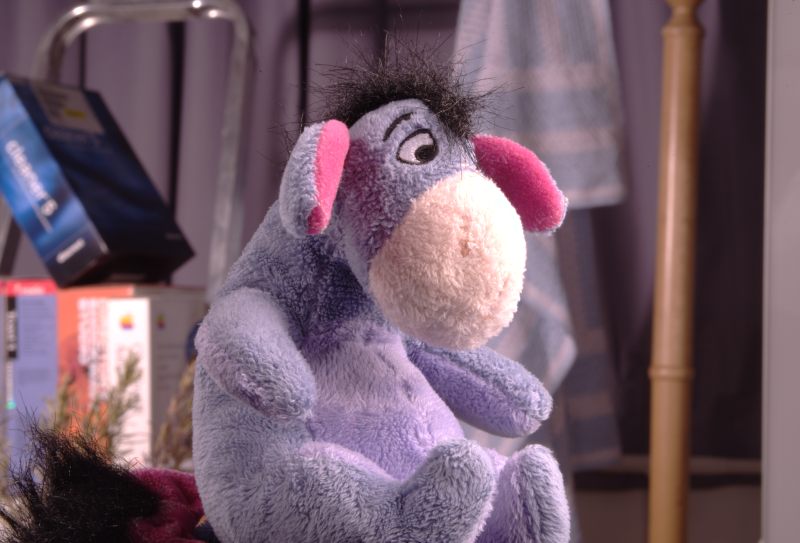
\includegraphics[width=0.2\textwidth]{GT24noflash.png}
    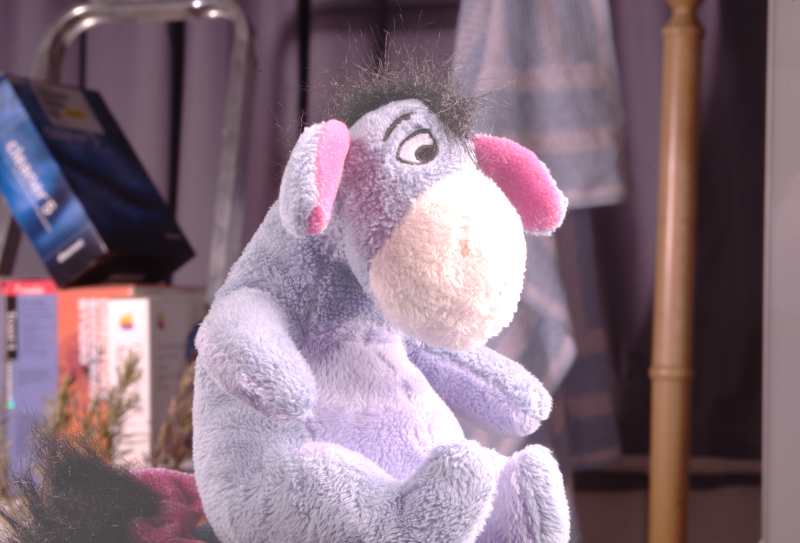
\includegraphics[width=0.2\textwidth]{GT24flash.png}
        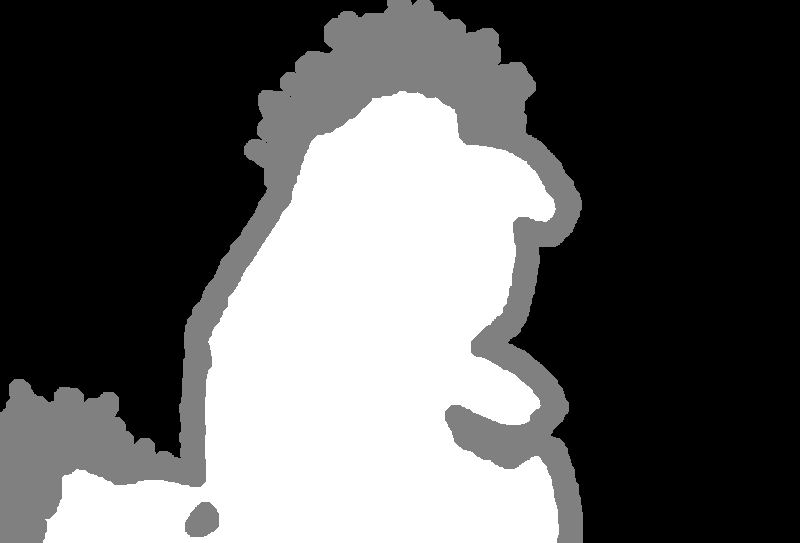
\includegraphics[width=0.2\textwidth]{GT24trimap.png}
            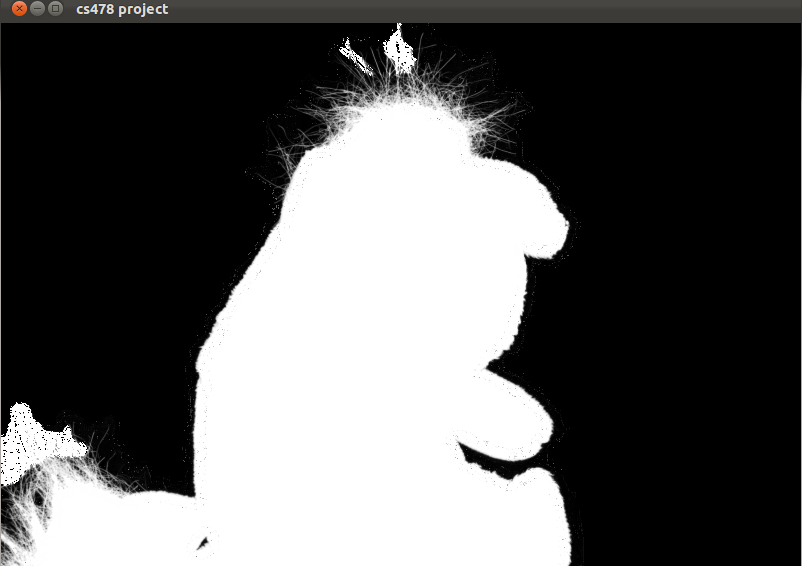
\includegraphics[width=0.2\textwidth]{nooo.png}
           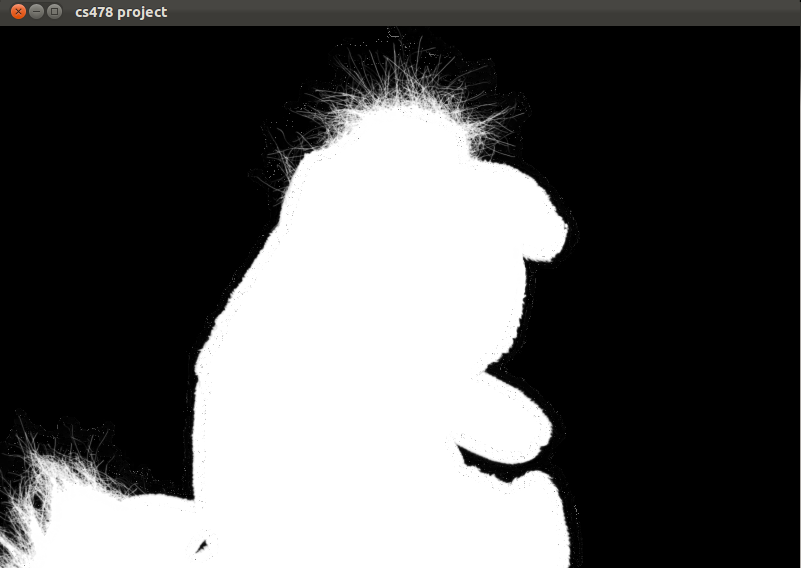
\includegraphics[width=0.2\textwidth]{alphamapp.png}
           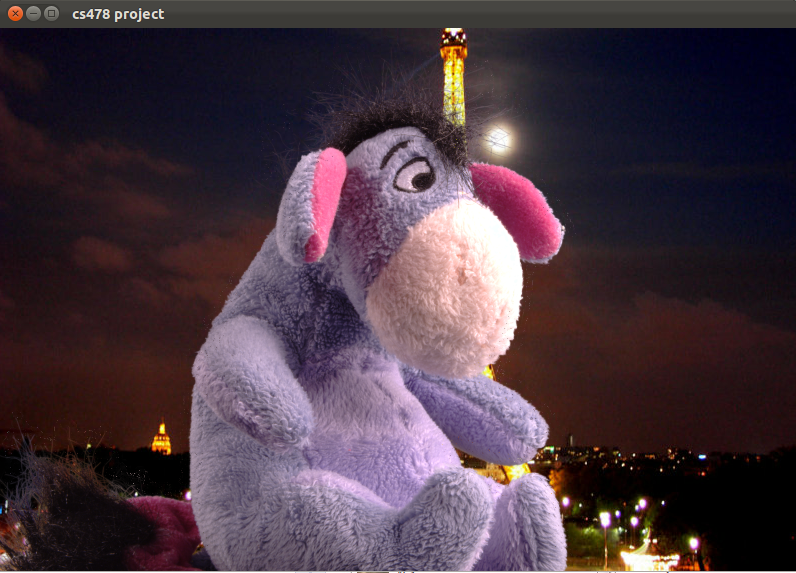
\includegraphics[width=0.2\textwidth]{igorparis.png}      
           \label{fig:igor}     
      \caption{Flash matting with a "fake" input. Top: Flash and No Flash. Mid: Trimap and failed alphamap. Bottom: Good alphamap and Composition.}
\end{figure}

The algorithm was first tested on a "fake" flash no-flash image. I downloaded an 100\% accurate alpha map with its no flash image from [4] and generated the flash image artificially by adding an equal amount of intensity from the alpha map to the no flash image. Figure 1 shows the result of the flash matting, where it can be seen the method performs very poor results in regions where there is a lot of half-transparent hair. It can also be seen that the algorithm gets much better results when its working from the foreground boundary than it does from the background boundary. 
\\
Although not mentioned in any paper and based on my results in figure 1, instead of working my way inwards the unknown region from both foreground and background region, I decided to try to only walk away from the foreground region since the results were more promising there. As can be seen in figure 1, the results are far more impressive with this traversing strategy than the ones mentioned in the papers. It still has some random spiky noise, which I tried to remove with a simple median filter (average every point with the neighboring median value). 
\\
To see if it actually works on a real image, I took a pair of photos with a Canon 550D camera. The results of the flash matting can be seen in figure 2. Once again there are spiky noise, that was reduced with a median filter.
\begin{figure}[h!]

  \centering
    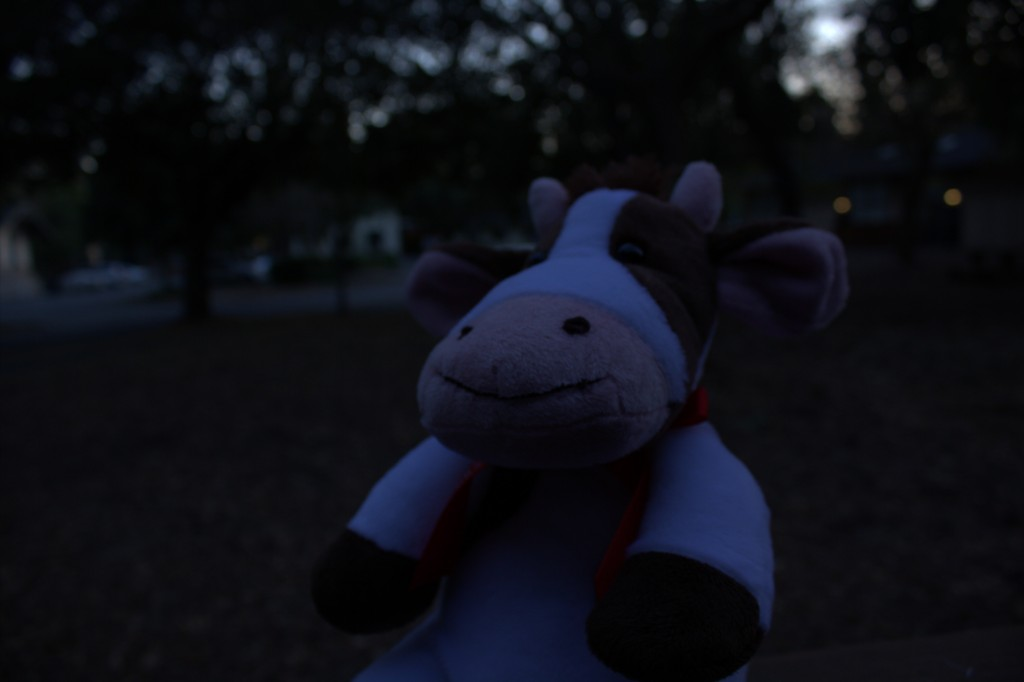
\includegraphics[width=0.2\textwidth]{cownoflash.jpg}
    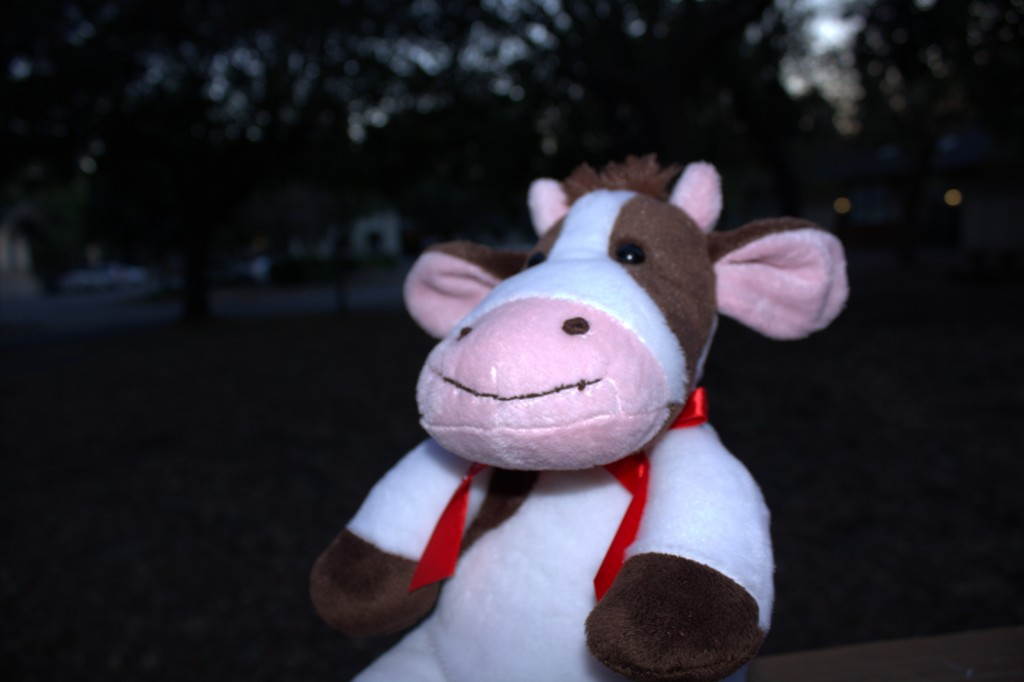
\includegraphics[width=0.2\textwidth]{cowflash.jpg}
        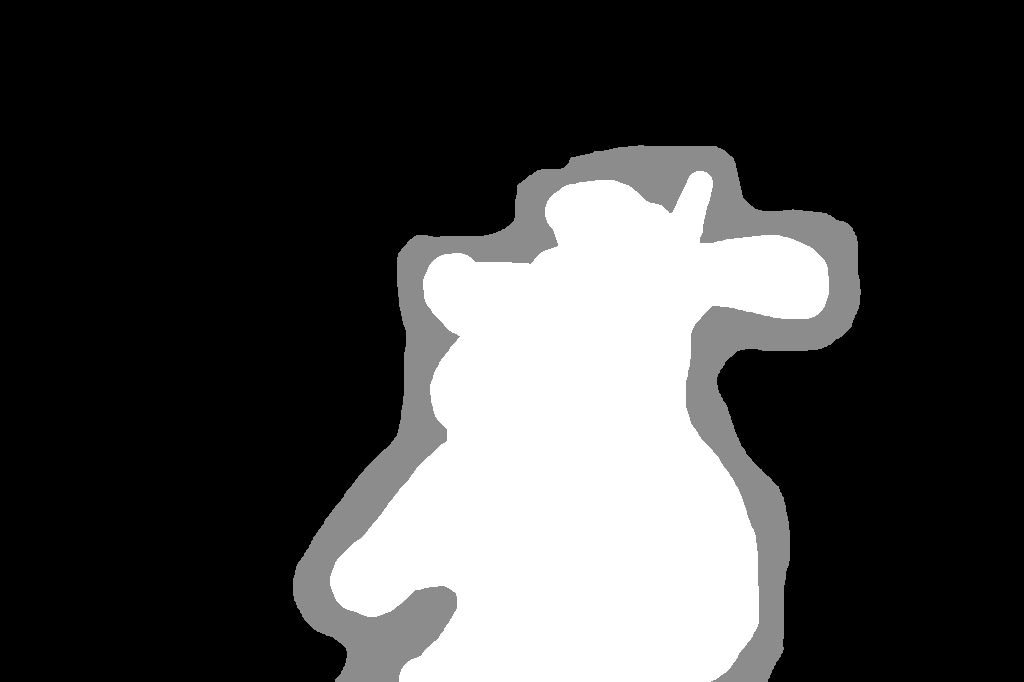
\includegraphics[width=0.2\textwidth]{trimap.png}
            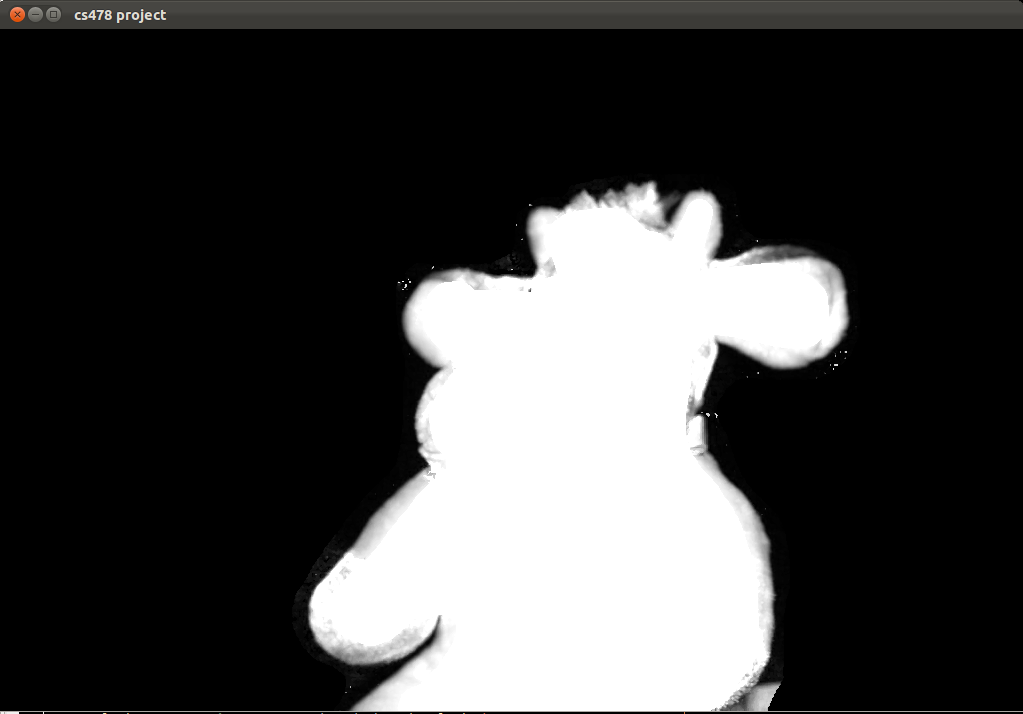
\includegraphics[width=0.2\textwidth]{cowalpha.png}
           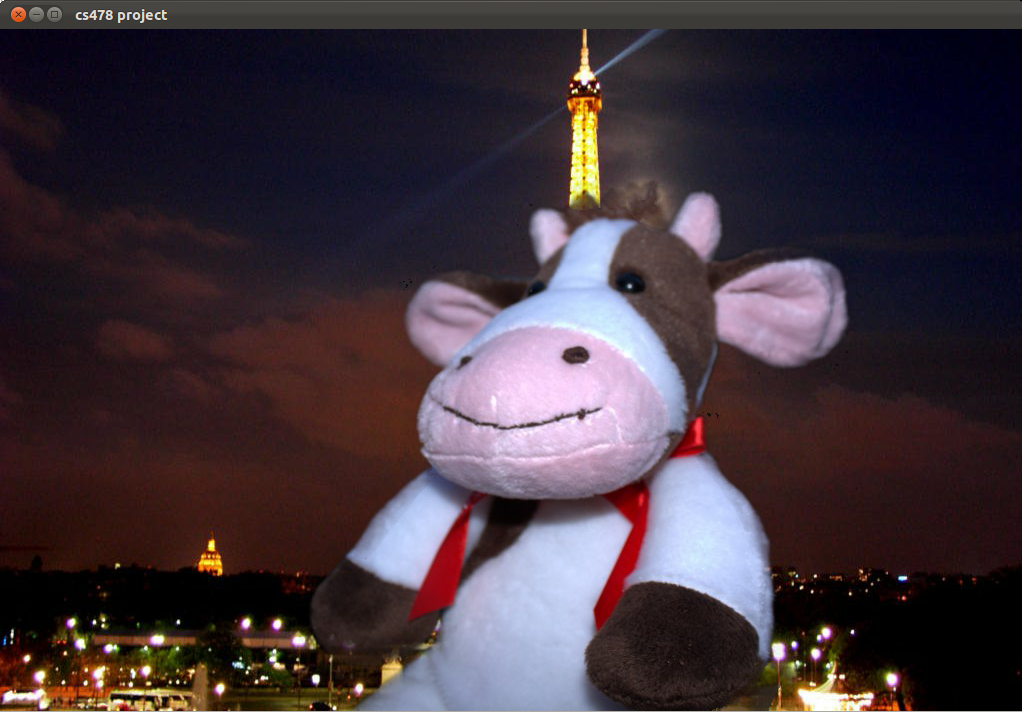
\includegraphics[width=0.35\textwidth]{cowparis.png}
      \caption{Flash matting with real input. Top: Flash and No Flash. Mid: Trimap and alphamap. Bottom: Composition.}
      \label{fig:cow}
\end{figure}

\section{Discussion}
\subsection{Time Complexity}
What surprised me during this project was that I underestimated the runtime of this algorithm. At a first glance at [3], it looked like a basic idea. The more I tried to understand the paper, the more I understood how bad the runtime scales if we want to increase accuracy. The timecomplexity depends on 3 parameters:
	\begin{equation}
O(N\cdot U\cdot A)
\label{eq:time}
	\end{equation}
	where $N$ is how many neighbor you take into account when calculating mean and covariance, $U$ is the number of unknown pixels in the image and $A$ which is the accuracy of the alpha solver (for simplicity, counted as number of iterations)
\subsection{Trimap}
As I briefly mentioned earler, I decided to use a hand made Trimap instead of the autogenerated one. The autogenerated trimap depends a lot on tweaking parameters, which makes it less "automatic". It has also a tendency of including unnecessary regions to the unknown region, parts that the human eye can tell easily divide either in foreground or background. As mentioned earlier, the time it takes to execute the program can be quite long at time, and to minimize parameter W in \ref{eq:time}, it makes sense to paint or select a small unknown area(if possible).
\subsection{Numerical errors}
The major time spent on this project was unfortunately spent on trying to figure out and resolve numerical errors. In equation \ref{eq:alpha}, nothing guarantees that $\alpha$ is in a nice range of $(0,1)$, and also the colors $F,B,F^d$ tends to "explode" and create huge artifacts and crashes in the code. It was also really hard to debug, because if a pixel failed at a certain position, then I had to track it backwards, which is painful the way the known pixels propagate over the unknown pixels.
\subsection{Tablet}
Even though first assignments were done on the NVIDIA tablet given in the class, I changed my mind halfway through the project and decided to not try and implement it on the tablet since I realized in my test cases that flash matting can be really sensitive to noise. Even though I used a fairly expensive Canon T2i camera, I still had a hard time producing a good flash/no flash image pair. Another reason is the long runtime. Even on my i7 cpu, it takes a lot of time to compute the alphamap since I didn't get any good results when lowering any of the variables in equation \ref{eq:time}.

\section{Further work}
It is unclear if the flash matting paper is using different clusters or not when approximating the Gaussian color distribution. It would be interesting to see how much better the solution would be if you properly divide distributions. I didn't have time to explore this at all and I have therefore no idea if it will improve the accuracy at all.

\section{Conclusion}
Even though I was a bit sceptic to the idea of flash matting halfway through the project when nothing worked and all I got was non-converging variables, it made a little more sense towards the end. What I found annoying about the flash matting paper[3] was that they don't mention how they solve numerical errors at all, something that would have helped me. It would also have been nice if they released their test data on their homepage, so you know what you are developing against in the beginning. My results were not perfect and had some smaller artefacts, but I still think they are okay in terms of how little manual work they need to be generated.

\section{References}
[1] A.R. Smith and J. F. Blinn. Blue Screen matting. In proceedings of SIGGRAPH 96\newline \newline
[2] Y.Y Chuang, B.Curless, D.H Salesin and R SZeliski. A baeysian approach to digital matting. In Proceedings of CVPR 2001.\newline \newline
[3] J. Sun, Y. Li, S.B Kang, H-Y Shum, Flash Matting. 2006\newline \newline
[4] http://www.alphamatting.com/

\end{document}